% !TEX encoding = UTF-8 Unicode
% !TEX TS-program = xelatex
\begin{QUESTIONS}
    \begin{QUESTION}
        \begin{ExamInfo}{94}{學測}{單選}{1}
        \end{ExamInfo}
        \begin{ExamAnsRateInfo}{73}{91}{78}{50}
        \end{ExamAnsRateInfo}
        \begin{QBODY}
            試問整數 43659 共有多少個不同的質因數? 
			\begin{QOPS} 
				\QOP 1 個 
				\QOP 2 個 
				\QOP 3 個 
				\QOP 4 個 
				\QOP 5 個
			\end{QOPS}
        \end{QBODY}
        \begin{QFROMS}
        \end{QFROMS}
        \begin{QTAGS}\QTAG{不是99課綱}\end{QTAGS}
        \begin{QANS}
            (3)
        \end{QANS}
        \begin{QSOLLIST}
        \end{QSOLLIST}
        \begin{QEMPTYSPACE}
        \end{QEMPTYSPACE}
    \end{QUESTION}
    \begin{QUESTION}
        \begin{ExamInfo}{94}{學測}{單選}{2}
        \end{ExamInfo}
        \begin{ExamAnsRateInfo}{78}{98}{89}{47}
        \end{ExamAnsRateInfo}
        \begin{QBODY}
            利用公式 $1^3 +2^3 + \cdots +n^3 = (\frac{n(n+1)}{2})^2$,可計算出 $(11)^3 + (12)^3 + \cdots +(20)^3$ 之值為 
		\begin{QOPS} 
			\QOP 41075
			\QOP 41095
			\QOP 41115	
			\QOP 41135	
			\QOP 41155
		\end{QOPS}
        \end{QBODY}
        \begin{QFROMS}
        \end{QFROMS}
        \begin{QTAGS}\QTAG{B2C1數列級數}\QTAG{B2C1-2級數}\end{QTAGS}
        \begin{QANS}
            (1)
        \end{QANS}
        \begin{QSOLLIST}
        \end{QSOLLIST}
        \begin{QEMPTYSPACE}
        \end{QEMPTYSPACE}
    \end{QUESTION}
    \begin{QUESTION}
        \begin{ExamInfo}{94}{學測}{單選}{3}
        \end{ExamInfo}
        \begin{ExamAnsRateInfo}{52}{82}{54}{20}
        \end{ExamAnsRateInfo}
        \begin{QBODY}
            台北銀行最早發行的樂透彩(俗稱小樂透)的玩法是「42 選 6」:購買者從 01 $\sim$ 42 中任選六個 號碼,當這六個號碼與開出的六個號碼完全相同(不計次序)時即得頭獎;台北銀行曾考慮改發行「39 選 5」的小小樂透:購買者從 01 $\sim$ 39 中任選五個號碼,如果這五個號碼與開出的五個號碼完全相同(不計次序)則得頭獎。假設原來的小樂透中頭獎的機率是 $R$,而曾考慮發行的小小樂透中頭獎的機率是 $r$。試問比值 $\frac{r}{R}$ 最接近下列哪個選項?
			\begin{QOPS}
				\QOP $3$
				\QOP $5$
				\QOP $7$
				\QOP $9$
				\QOP $11$
			\end{QOPS}
        \end{QBODY}
        \begin{QFROMS}
        \end{QFROMS}
        \begin{QTAGS}\QTAG{B2C3機率}\QTAG{B2C3-2機率的定義與性質}\end{QTAGS}
        \begin{QANS}
            (4)
        \end{QANS}
        \begin{QSOLLIST}
        \end{QSOLLIST}
        \begin{QEMPTYSPACE}
        \end{QEMPTYSPACE}
    \end{QUESTION}
    \begin{QUESTION}
        \begin{ExamInfo}{94}{學測}{單選}{4}
        \end{ExamInfo}
        \begin{ExamAnsRateInfo}{32}{65}{21}{10}
        \end{ExamAnsRateInfo}
        \begin{QBODY}
            設 $a, b$ 為正實數,已知 $\log_7 a = 11$,$\log_7 b = 13$ ;試問 $\log_7 (a + b)$ 之值最接近下列哪個選項? 
			\begin{QOPS} 
				\QOP 12 
				\QOP 13 
				\QOP 14 
				\QOP 23 
				\QOP 24
			\end{QOPS}
        \end{QBODY}
        \begin{QFROMS}
        \end{QFROMS}
        \begin{QTAGS}\QTAG{B1C3-3對數}\QTAG{B1C3指對數函數}\QTAG{對數律}\end{QTAGS}
        \begin{QANS}
            (2)
        \end{QANS}
        \begin{QSOLLIST}
        \end{QSOLLIST}
        \begin{QEMPTYSPACE}
        \end{QEMPTYSPACE}
    \end{QUESTION}
    \begin{QUESTION}
        \begin{ExamInfo}{94}{學測}{單選}{5}
        \end{ExamInfo}
        \begin{ExamAnsRateInfo}{8}{10}{7}{7}
        \end{ExamAnsRateInfo}
        \begin{QBODY}
            某校高一第一次段考數學成績不太理想,多數同學成績偏低;考慮到可能是同學們適應不良所致,數學老師決定將每人的原始成績取平方根後再乘以 10 作為正式紀錄的成績。今隨機抽選 100 位同學,發現調整後的成績其平均為 65 分,標準差為 15 分;試問這 100 位同學未調整前的成績之平均 $M$ 介於哪兩個連續正整數之間? 
			\begin{QOPS} 
				\QOP $40 \leq M <41$ 
				\QOP $41\leq  M<42$ 
				\QOP$ 42 \leq M<43$        
				\QOP $43 \leq M<44$        
				\QOP $44\leq  M<45$
			\end{QOPS}
        \end{QBODY}
        \begin{QFROMS}
        \end{QFROMS}
        \begin{QTAGS}\QTAG{平均數}\QTAG{B2C4-1一維數據分析}\QTAG{B2C4數據分析}\QTAG{標準差}\end{QTAGS}
        \begin{QANS}
            (5)
        \end{QANS}
        \begin{QSOLLIST}
        \end{QSOLLIST}
        \begin{QEMPTYSPACE}
        \end{QEMPTYSPACE}
    \end{QUESTION}
\end{QUESTIONS}
\begin{QUESTIONS}
    \begin{QUESTION}
        \begin{ExamInfo}{94}{學測}{多選}{6}
        \end{ExamInfo}
        \begin{ExamAnsRateInfo}{53}{81}{52}{26}
        \end{ExamAnsRateInfo}
        \begin{QBODY}
            如右圖所示,兩射線 $\lvec{OA}$ 與 $\lvec{OB}$ 交於 $O$ 點,試問下列選項中哪些向量的終點會落在陰影區域內?
			\begin{QOPS} 
				\QOP $\lvec{OA} + 2\lvec{OB}$
				\QOP  $\frac{3}{4}\lvec{OA} + \frac{1}{3} \lvec{OB}$ 
				\QOP $\frac{3}{4}\lvec{OA} - \frac{1}{3}\lvec{OB}$ 
				\QOP $\frac{3}{4}\lvec{OA} + \frac{1}{5} \lvec{OB}$ 
				\QOP $\frac{3}{4}\lvec{OA} - \frac{1}{5} \lvec{OB}$
			\end{QOPS}
			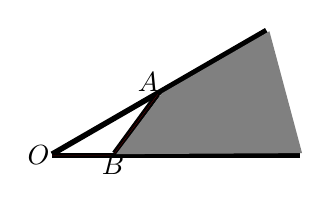
\begin{tikzpicture}[scale=.8]
				\begin{scope}[inner sep=0pt]
				\node (vO) at (0,0) {};
				\node[anchor = east] (tO) at (vO) {$O$};
				\node (vB) at (0:1) {};
				\node[anchor = north] (tB) at (vB) {$B$};
				\node (vD) at (0:4) {};
				\node (vA) at (30:2) {};
				\node[anchor = south  east] (tA) at (vA) {$A$};
				\node (vC) at (30:4) {};
				\draw[line width=2pt] (vA) to (vB);
				\draw[line width=2pt] (vO) to (vD);
				\draw[line width=2pt] (vO) to (vC);
				\fill[red] (vA) -- (vB) -- (vO);
				\fill[gray]  (1:1.05) -- (.5:4) -- (29.5:4) -- (29:2.03);
				\end{scope}
			\end{tikzpicture}
        \end{QBODY}
        \begin{QFROMS}
        \end{QFROMS}
        \begin{QTAGS}\QTAG{線性組合}\QTAG{B3C3-1平面向量的表示法}\QTAG{B3C3平面向量}\end{QTAGS}
        \begin{QANS}
            (1)(2)
        \end{QANS}
        \begin{QSOLLIST}
        \end{QSOLLIST}
        \begin{QEMPTYSPACE}
        \end{QEMPTYSPACE}
    \end{QUESTION}
    \begin{QUESTION}
        \begin{ExamInfo}{94}{學測}{多選}{7}
        \end{ExamInfo}
        \begin{ExamAnsRateInfo}{56}{87}{59}{22}
        \end{ExamAnsRateInfo}
        \begin{QBODY}
            如右圖所示,坐標平面上一鳶形 $ABCD$, 其中 $A,C$ 在 $y$-軸上, $B$, $D$ 在 $x$-軸上, 且 $\overline{AB} = \overline{AD} =2$, $\overline{BC} = \overline{CD} =4$, $\overline{AC} =5$。 令 $m_{AB}$, $m_{BC}$, $m_{CD}$,  $m_{DA}$ 分別表直線 $AB$, $BC$, $CD$, $DA$ 之斜率。試問以下哪些敘述成立? 
			\begin{QOPS} 
				\QOP 此四數值中以 $m_{AB}$ 為最大 
				\QOP 此四數值中以 $m_{BC}$ 為最小 
				\QOP $m_{BC}= - m_{CD}$  
				\QOP $m_{AB} \times m_{BC} =-1$ 
				\QOP $m_{CD} +m_{DA} >0$
			\end{QOPS}
			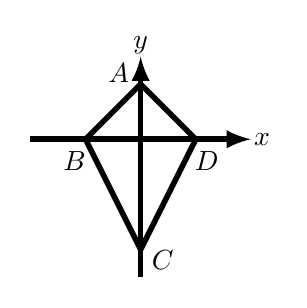
\begin{tikzpicture}[scale=.7]
				\pgfsetlinewidth{2pt}
				\node at (0,1.7) {$y$};
				\node at (2.2,0) {$x$};
				\node at (1.2,-.4) {$D$};
				\node at (-1.2,-.4) {$B$};
				\node at (-.4,1.2) {$A$};
				\node at (.4,-2.2) {$C$};
				\draw (1,0) to (0,1);
				\draw (-1,0) to (0,1);
				\draw (1,0) to (0,-2);
				\draw (-1,0) to (0,-2);
				\pgfsetarrowsend{latex}
				\draw (-2,0) to[->] (2,0);
				\draw (0,-2.5) to[->] (0,1.5);
			\end{tikzpicture}
        \end{QBODY}
        \begin{QFROMS}
        \end{QFROMS}
        \begin{QTAGS}\QTAG{B3C2-1直線方程式及其圖形}\QTAG{B3C2直線與圓}\end{QTAGS}
        \begin{QANS}
            (2)(3)(5)
        \end{QANS}
        \begin{QSOLLIST}
        \end{QSOLLIST}
        \begin{QEMPTYSPACE}
        \end{QEMPTYSPACE}
    \end{QUESTION}
    \begin{QUESTION}
        \begin{ExamInfo}{94}{學測}{多選}{8}
        \end{ExamInfo}
        \begin{ExamAnsRateInfo}{34}{67}{22}{13}
        \end{ExamAnsRateInfo}
        \begin{QBODY}
            假設坐標空間中三相異平面 $E_1$, $E_2$, $E_3$ 皆通過 $(-1,2,0)$ 與 $(3,0,2)$ 兩點,試問以下哪些點也同時在此三平面上? 
			\begin{QOPS} 
				\QOP (2,2,2) 
				\QOP (1,1,1) 
				\QOP (4,-2,2) 
				\QOP (-2,4,0) 
				\QOP (-5,-4,-2)
			\end{QOPS}
        \end{QBODY}
        \begin{QFROMS}
        \end{QFROMS}
        \begin{QTAGS}\QTAG{B4C2空間中的平面與直線}\QTAG{B4C2-2空間直線方程式}\end{QTAGS}
        \begin{QANS}
            (2)
        \end{QANS}
        \begin{QSOLLIST}
        \end{QSOLLIST}
        \begin{QEMPTYSPACE}
        \end{QEMPTYSPACE}
    \end{QUESTION}
    \begin{QUESTION}
        \begin{ExamInfo}{94}{學測}{多選}{9}
        \end{ExamInfo}
        \begin{ExamAnsRateInfo}{37}{69}{32}{10}
        \end{ExamAnsRateInfo}
        \begin{QBODY}
            若 $0 < \theta < \frac{\pi}{4}$ ,試問以下哪些選項恆成立? 
			\begin{QOPS} 
				\QOP	$\sin \theta < \cos \theta$	
				\QOP	$\tan \theta < \sin \theta$ 
				\QOP $\cos \theta < \tan \theta$ 
				\QOP $\sin{2\theta} <\cos{2\theta}$ 
				\QOP $\tan{\frac{\theta}{2}} <\frac{1}{2} \tan \theta$
			\end{QOPS}
        \end{QBODY}
        \begin{QFROMS}
        \end{QFROMS}
        \begin{QTAGS}\QTAG{B3C1-1簡單的三角函數}\QTAG{B3C1三角}\end{QTAGS}
        \begin{QANS}
            (1)(5)
        \end{QANS}
        \begin{QSOLLIST}
        \end{QSOLLIST}
        \begin{QEMPTYSPACE}
        \end{QEMPTYSPACE}
    \end{QUESTION}
    \begin{QUESTION}
        \begin{ExamInfo}{94}{學測}{多選}{10}
        \end{ExamInfo}
        \begin{ExamAnsRateInfo}{29}{47}{23}{17}
        \end{ExamAnsRateInfo}
        \begin{QBODY}
            設 $F_1$ 與 $F_2$ 為坐標平面上雙曲線 $\Gamma : \frac{x^2}{9} -\frac{y^2}{16} =1$ 的兩個焦點,$P$ 為 $\Gamma$ 上一點,使得此三點構成一等腰三角形。試問以下哪些值可能是這些等腰三角形的週長? 
			\begin{QOPS} 
				\QOP 20	
				\QOP 24 
				\QOP 28 
				\QOP 32	
				\QOP 36 。
			\end{QOPS}
        \end{QBODY}
        \begin{QFROMS}
        \end{QFROMS}
        \begin{QTAGS}\QTAG{B4C4-3雙曲線}\QTAG{B4C4二次曲線}\QTAG{圖形}\end{QTAGS}
        \begin{QANS}
            (2)(5)
        \end{QANS}
        \begin{QSOLLIST}
        \end{QSOLLIST}
        \begin{QEMPTYSPACE}
        \end{QEMPTYSPACE}
    \end{QUESTION}
    \begin{QUESTION}
        \begin{ExamInfo}{94}{學測}{多選}{11}
        \end{ExamInfo}
        \begin{ExamAnsRateInfo}{32}{51}{30}{15}
        \end{ExamAnsRateInfo}
        \begin{QBODY}
            設 $S$ 為空間中一球面, $\overline{AB}$ 為其一直徑,且 $\overline{AB} =10$。若 $ P$ 為空間中一點,使得 $\overline{PA} + \overline{PB} = 14$, 則 $P$ 點的位置可能落在哪裡? 
			\begin{QOPS} 
				\QOP 線段 $\overline{AB}$ 上; 
				\QOP 直線 $AB$ 上,但不在線段 $\overline{AB}$ 上; 
				\QOP	球面 $S$ 上; 
				\QOP 球 $S$ 的內部,但不在線段 $AB$ 上; 
				\QOP 球 $S$ 的外部,但不在直線 AB 上。
			\end{QOPS}
        \end{QBODY}
        \begin{QFROMS}
        \end{QFROMS}
        \begin{QTAGS}\QTAG{不是99課綱}\end{QTAGS}
        \begin{QANS}
            (2)(3)(4)(5)
        \end{QANS}
        \begin{QSOLLIST}
        \end{QSOLLIST}
        \begin{QEMPTYSPACE}
        \end{QEMPTYSPACE}
    \end{QUESTION}
\end{QUESTIONS}
\begin{QUESTIONS}
    \begin{QUESTION}
        \begin{ExamInfo}{94}{學測}{填充}{A}
        \end{ExamInfo}
        \begin{ExamAnsRateInfo}{69}{92}{82}{33}
        \end{ExamAnsRateInfo}
        \begin{QBODY}
            若多項式 $x^2 +x+2$ 能整除 $x^5 + x^4 +x^3 +px^2 +2x+q$,
			則 $p= \TCNBOX{\TCN}$、 $q=\TCNBOX{\TCN}$ 。
        \end{QBODY}
        \begin{QFROMS}
        \end{QFROMS}
        \begin{QTAGS}\QTAG{B1C2多項式函數}\QTAG{多項式除法}\QTAG{B1C2-2多項式的運算與應用}\end{QTAGS}
        \begin{QANS}
            $p=3,q=8$
        \end{QANS}
        \begin{QSOLLIST}
        \end{QSOLLIST}
        \begin{QEMPTYSPACE}
        \end{QEMPTYSPACE}
    \end{QUESTION}
    \begin{QUESTION}
        \begin{ExamInfo}{94}{學測}{填充}{B}
        \end{ExamInfo}
        \begin{ExamAnsRateInfo}{39}{78}{34}{5}
        \end{ExamAnsRateInfo}
        \begin{QBODY}
            在坐標平面上,正方形 $ABCD$ 的四個頂點坐標分別為 $A(0,1)$, $B(0,0)$, $C(1,0)$, $D(1,1)$。設 $P$ 為 正方形 $ABCD$ 內部的一點,若 $\triangle PDA$ 與 $\triangle PBC$ 的面積比為 $1:2$,且 $\triangle PAB$ 與 $\triangle PCD$ 的面積比為 $2:3$,則 $P$ 點的坐標為 $\TCNBOX{ (\FR{\TCN}{\TCN}, \FR{\TCN}{\TCN})}$。
        \end{QBODY}
        \begin{QFROMS}
        \end{QFROMS}
        \begin{QTAGS}\QTAG{面積}\QTAG{B3C3-3面積與二階行列式}\QTAG{B3C3-1平面向量的表示法}\QTAG{B3C3平面向量}\QTAG{線性組合}\end{QTAGS}
        \begin{QANS}
            $(\frac{2}{5},\frac{2}{3})$
        \end{QANS}
        \begin{QSOLLIST}
        \end{QSOLLIST}
        \begin{QEMPTYSPACE}
        \end{QEMPTYSPACE}
    \end{QUESTION}
    \begin{QUESTION}
        \begin{ExamInfo}{94}{學測}{填充}{C}
        \end{ExamInfo}
        \begin{ExamAnsRateInfo}{51}{80}{51}{22}
        \end{ExamAnsRateInfo}
        \begin{QBODY}
            在數線上有一個運動物體從原點出發,在此數線上跳動,每次向正方向或負方向跳 1 個單 位,跳動過程可重複經過任何一點。若經過 6 次跳動後運動物體落在點 $+4$ 處,則此運動物體共有 
			$\TCNBOX{\TCN}$ 種不同的跳動方法。
        \end{QBODY}
        \begin{QFROMS}
        \end{QFROMS}
        \begin{QTAGS}\QTAG{B2C2-2排列}\QTAG{含相同物排列}\QTAG{B2C2排列組合}\end{QTAGS}
        \begin{QANS}
            $6$
        \end{QANS}
        \begin{QSOLLIST}
        \end{QSOLLIST}
        \begin{QEMPTYSPACE}
        \end{QEMPTYSPACE}
    \end{QUESTION}
    \begin{QUESTION}
        \begin{ExamInfo}{94}{學測}{填充}{D}
        \end{ExamInfo}
        \begin{ExamAnsRateInfo}{21}{48}{14}{1}
        \end{ExamAnsRateInfo}
        \begin{QBODY}
            設複數 $z=1-i$;若 $1+z+z^2 + \cdots +z^9 =a+bi$,其中 $a$, $b$ 為實數,則$ a= \TCNBOX{\TCN\TCN}$ 、 $b=\TCNBOX{\TCN\TCN}$ 。
        \end{QBODY}
        \begin{QFROMS}
        \end{QFROMS}
        \begin{QTAGS}\QTAG{B2C1數列級數}\QTAG{複數}\QTAG{B2C1-2級數}\QTAG{B1C2多項式函數}\QTAG{B1C2-3多項式方程式}\QTAG{等比級數}\end{QTAGS}
        \begin{QANS}
            $32, -1$
        \end{QANS}
        \begin{QSOLLIST}
        \end{QSOLLIST}
        \begin{QEMPTYSPACE}
        \end{QEMPTYSPACE}
    \end{QUESTION}
    \begin{QUESTION}
        \begin{ExamInfo}{94}{學測}{填充}{E}
        \end{ExamInfo}
        \begin{ExamAnsRateInfo}{13}{36}{3}{0}
        \end{ExamAnsRateInfo}
        \begin{QBODY}
            設 $O$ 為坐標平面上的原點,$P$ 點坐標為 $(2, 1)$;若 $A$, $B$ 分別是正 $x$-軸及正 $y$-軸上的點,使得 $PA \bot PB$ ,則 $\triangle OAB$ 面積的最大可能值為 $\TCNBOX{\FR{\TCN\TCN}{\TCN\TCN}}$。
        \end{QBODY}
        \begin{QFROMS}
        \end{QFROMS}
        \begin{QTAGS}\QTAG{面積}\QTAG{B3C3-2平面向量的內積}\QTAG{B3C3平面向量}\QTAG{B3C3-3面積與二階行列式}\end{QTAGS}
        \begin{QANS}
            $\frac{25}{16}$
        \end{QANS}
        \begin{QSOLLIST}
        \end{QSOLLIST}
        \begin{QEMPTYSPACE}
        \end{QEMPTYSPACE}
    \end{QUESTION}
    \begin{QUESTION}
        \begin{ExamInfo}{94}{學測}{填充}{F}
        \end{ExamInfo}
        \begin{ExamAnsRateInfo}{17}{38}{8}{5}
        \end{ExamAnsRateInfo}
        \begin{QBODY}
            如右圖所示,在 $\triangle ABC$ 中, $\angle BAC$ 的平分線 $AD$ 交對邊 $BC$ 於$D$;已知 $\overline{BD}=3$, $\overline{DC} = 6$ 且 $\overline{AB} = \overline{AD}$ ,則 $\cos \angle BAD$ 之值為 $\TCNBOX{\FR{\TCN}{\TCN}}$ 。
			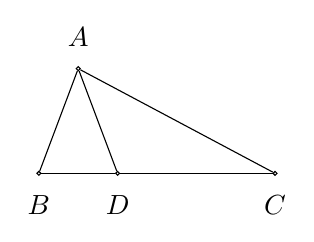
\begin{tikzpicture}[inner sep = 0pt]
				\tikzstyle{vnode}=[draw,circle,inner sep=.5pt];
				\node[vnode]  (vB) at (0,0) {};
				\node  (tB) at (0,-.4) {$B$};
				\node[vnode]  (vD) at (1,0) {};
				\node  (tD) at (1,-.4) {$D$};
				\node[vnode]  (vC) at (3,0) {};
				\node  (tC) at (3,-.4) {$C$};
				\node[vnode]  (vA) at (.5,1.33) {};
				\node  (tA) at (.5,1.73) {$A$}; 
				\draw (vB) to (vD);
				\draw (vC) to (vD);
				\draw (vA) to (vD);
				\draw (vB) to (vA);
				\draw (vC) to (vA);
			\end{tikzpicture}
        \end{QBODY}
        \begin{QFROMS}
        \end{QFROMS}
        \begin{QTAGS}\QTAG{B3C1-3正弦定理與餘弦定理}\QTAG{B3C1三角}\end{QTAGS}
        \begin{QANS}
            $\dfrac{3}{4}$
        \end{QANS}
        \begin{QSOLLIST}
        \end{QSOLLIST}
        \begin{QEMPTYSPACE}
        \end{QEMPTYSPACE}
    \end{QUESTION}
    \begin{QUESTION}
        \begin{ExamInfo}{94}{學測}{填充}{G}
        \end{ExamInfo}
        \begin{ExamAnsRateInfo}{12}{24}{8}{4}
        \end{ExamAnsRateInfo}
        \begin{QBODY}
            在坐標平面上,過 $F(1,0)$ 的直線交拋物線 $\Gamma : y^2 = 4x$ 於 $P$, $Q$ 兩點,
			其中 $P$ 在上半平面,且知 $2\overline{PF} = 3\overline{QF}$ ,
			則 $P$ 點的 $x$-坐標為 
			$\TCNBOX{\FR{\TCN}{\TCN}}$。
        \end{QBODY}
        \begin{QFROMS}
        \end{QFROMS}
        \begin{QTAGS}\QTAG{B4C4二次曲線}\QTAG{B4C4-1拋物線}\end{QTAGS}
        \begin{QANS}
            $\frac{3}{2}$
        \end{QANS}
        \begin{QSOLLIST}
        \end{QSOLLIST}
        \begin{QEMPTYSPACE}
        \end{QEMPTYSPACE}
    \end{QUESTION}
    \begin{QUESTION}
        \begin{ExamInfo}{94}{學測}{填充}{H}
        \end{ExamInfo}
        \begin{ExamAnsRateInfo}{32}{66}{25}{5}
        \end{ExamAnsRateInfo}
        \begin{QBODY}
            設 $x$ 為一正實數且滿足 $x\cdot 3^x =3^{18}$;若 $x$ 落在連續正整數 $k$ 與 $k+1$ 之間,則$k= \TCNBOX{\TCN\TCN}$。
        \end{QBODY}
        \begin{QFROMS}
        \end{QFROMS}
        \begin{QTAGS}\QTAG{B1C2多項式函數}\QTAG{B1C2-3多項式方程式}\QTAG{B1C3-2指數函數}\QTAG{B1C3指對數函數}\QTAG{勘根定理}\end{QTAGS}
        \begin{QANS}
            $15$
        \end{QANS}
        \begin{QSOLLIST}
        \end{QSOLLIST}
        \begin{QEMPTYSPACE}
        \end{QEMPTYSPACE}
    \end{QUESTION}
    \begin{QUESTION}
        \begin{ExamInfo}{94}{學測}{填充}{I}
        \end{ExamInfo}
        \begin{ExamAnsRateInfo}{26}{63}{13}{2}
        \end{ExamAnsRateInfo}
        \begin{QBODY}
            如右圖所示,$ABCD-EFGH$ 為邊長等於 1 之 正立方體。
			若 $P$ 點在立方體之內部且滿足 
			$\lvec{AP} =\frac{3}{4} \lvec{AB} +\frac{1}{2} \lvec{AD} +\frac{2}{3} \lvec{AE}$,則 $P$ 點至直線
			$\overline{AB}$ 之距離為 
			$\TCNBOX{\FR{\TCN}{\TCN}}$ 。
			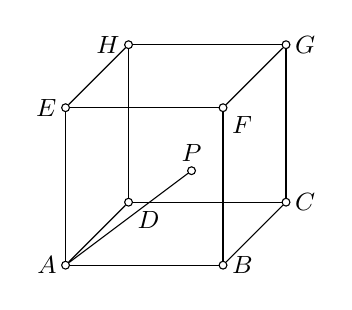
\begin{tikzpicture}
				\begin{scope}
				\small
				\tikzstyle{vnode}=[draw,circle,inner sep =1pt];
				\node[vnode] (v000) at (0,0) {};
				\node[anchor =north west] (t000) at (v000) {$D$};
				\node[vnode] (v001) at (0,2) {$$};
				\node[anchor =east] (t000) at (v001) {$H$};
				\node[vnode] (v011) at (2,2) {$$};
				\node[anchor =west] (t011) at (v011) {$G$};
				\node[vnode] (v010) at (2,0) {$$};
				\node[anchor =west] (t010) at (v010) {$C$};
				\node[vnode] (v100) at (-.8,-.8) {$$};
				\node[anchor =east] (t100) at (v100) {$A$};
				\node[vnode] (v101) at (-.8,1.2) {$$};
				\node[anchor =east] (t101) at (v101) {$E$};
				\node[vnode] (v111) at (1.2,1.2) {$$};
				\node[anchor =north west] (t111) at (v111) {$F$};
				\node[vnode] (v110) at (1.2,-0.8) {$$};
				\node[anchor =west] (t110) at (v110) {$B$};
				\node[vnode] (vP) at (.8,.4) {$$};
				\node[anchor =south] (tP) at (vP) {$P$};
				\draw (v100) to[dashed] (vP);
				\foreach \i in {01,10,11}{
						\draw (v0\i) to (v1\i);
						\draw (v\i  0) to (v\i 1);
				}
				\draw (v000) to[dashed] (v100);
				\draw (v000) to[dashed] (v010);
				\draw (v000) to[dashed] (v001);
				\draw (v001) to (v011);
				\draw (v100) to (v110);
				\draw (v101) to (v111);
				\end{scope}
			\end{tikzpicture}
        \end{QBODY}
        \begin{QFROMS}
        \end{QFROMS}
        \begin{QTAGS}\QTAG{B4C1-1空間概念}\QTAG{B4C1空間向量}\end{QTAGS}
        \begin{QANS}
            $\dfrac{5}{6}$
        \end{QANS}
        \begin{QSOLLIST}
        \end{QSOLLIST}
        \begin{QEMPTYSPACE}
        \end{QEMPTYSPACE}
    \end{QUESTION}
\end{QUESTIONS}
